\documentclass[10pt]{article}

\def\Type{LessonCaelan}
\def\TypeNum{Lesson 15}
\def\TypeTitle{Net Change, Area \& Definite Integrals\\Solutions }
\def\Semester{Fall 2021} %Not Used 
\def\Course{MATH 1190 \& 1210}
\def\Targets{  {\bf\color{Fuchsia}I1} }

\usepackage{preambleDJ}



%%%%%%%%%%%% BEGIN DOCUMENT %%%%%%%%%%%%%%%
%%%%%%%%%%%% BEGIN DOCUMENT %%%%%%%%%%%%%%%
%%%%%%%%%%%% BEGIN DOCUMENT %%%%%%%%%%%%%%%
%%%%%%%%%%%% BEGIN DOCUMENT %%%%%%%%%%%%%%%
%%%%%%%%%%%% BEGIN DOCUMENT %%%%%%%%%%%%%%%



\begin{document}

\pagestyle{otherpages}
\thispagestyle{firstpage}
\vs{.65}

\textbf{Intended Learning Outcomes}
After this lesson, you will be able to 

\itemC{
    \item Estimate definite integrals using rectangles of equal width. (\target{I1})
    \item Explain the meaning of a definite integral of a function in context, including determining the units of the integral. (\target{I1})
    \item Write mathematical expressions involving definite integrals to represent a given scenario. (\target{I1})
}

\vspace{-0.25cm}

\hrulefill\\

\vs{-.2}
During our first lesson of the semester, we asked ``how are slope, rate of change, and net change related?". So far, we've discovered that slope and AROC are identical in a linear relationship, and that the slope of a tangent line is identical to IROC. However, we have not meaningfully related net change to any of these quantities.\\

Now that we've extensively developed a tool $-$ the derivative $-$ that can measure slopes \& IROC, we can begin to make better sense of the relationship between these quantities and net change. In this lesson, we will begin by using IROC estimating net change, and then introduce a new tool that can measure net change directly.\\

{\example}\ltrm{\target{I1}} Similarly to the online pre-class assignment, $x(t)$ represents the position (in meters) of the object from the origin at time $t$ (in seconds).  The graph of the velocity $x^{\prime}(t)= v(t)$ (in m/sec) of an object is given below, where $t$ is the time (in sec) since the object's movements were initially measured. 
    \begin{enumerate}
    \item[(a)] Estimate the net change $\Delta x$ in the position of the object between $2$ and $4$ seconds after measurements were initially taken.  Recall that {\em Distance = Rate $\times$ Time} (if {\em Rate} is constant).
    \end{enumerate}
%
\vs{-.2}\hs{-.5}\mpageTth{.3}{.6}{.3}{\flushleft
%{ % Start a local group
  %\captionsetup{justification=raggedright, singlelinecheck=false}
\begin{minipage}{1.875in}
\centering
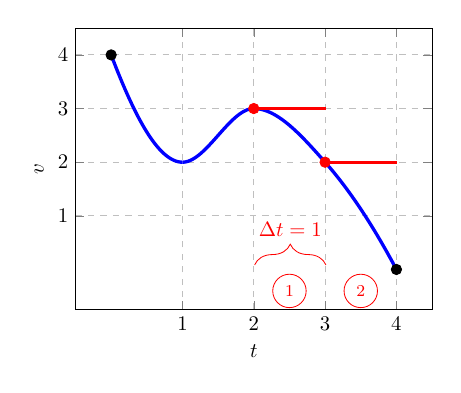
\begin{tikzpicture}[scale=0.75]
          \begin{axis}[
        %    axis y line = left,
        %    axis x line = bottom,
            xlabel = {$t$},
            ylabel = {$v$},
            xtick       = {1,2,3,4},
            xticklabels = {$1$,$2$,$3$,$4$},
            ytick       = {-2,-1,1,2,3,4,5,6},
            yticklabels = {$-2$,$-1$,$1$,$2$,$3$,$4$,$5$,$6$},
            samples     = 320,
            domain      = 0:4,
            %restrict y to domain=-5:5,
            xmin = -0.5, xmax = 4.5,
            ymin = -0.75, ymax = 4.5,
            width=3in,height=2.5in,
            grid=both, grid style=dashed
          ]
               \addplot[blue, ultra thick, mark=none, smooth, domain=0:1]  {4-7* x/2 + x^2 + x^3/2};
          \addplot[blue, ultra thick, mark=none, smooth, domain=1:2]  {7 - 12*x + 9*x^2 - 2*x^3};
          \addplot[blue, ultra thick, mark=none, smooth, domain=2:3]  {-7 + 12*x - 9/2* x^2 + x^3/2};
          \addplot[blue, ultra thick, mark=none, smooth, domain=3:4]  {2 + 3*x/2 - x^2/2};
         %
         \filldraw (0,4) circle (2.5pt);
         %
         \filldraw (4,0) circle (2.5pt);
\draw [decorate,decoration={brace,amplitude=+10pt},xshift=0.4pt,yshift=-0.4pt, red](2,.1) -- (3,.1) node[red,midway,yshift=0.6cm] { $\Delta t=1$};
\node[circle,draw, red]  at (2.5,-.4){\footnotesize $1$};
\node[circle,draw, red]  at (3.5,-.4){\footnotesize $2$};
 \addplot[red, ultra thick, mark=none, smooth, domain=2:3]  {3};
          \filldraw[red] (2,3) circle (2.5pt);
           \addplot[red, ultra thick, mark=none, smooth, domain=3:4]  {2};
          \filldraw[red] (3,2) circle (2.5pt);
         \end{axis}
    \end{tikzpicture}
       \vs{-.1} \captionof*{figure}{\bf \footnotesize{ Approach $\#1$:\\Left endpoints}}
       \end{minipage}
 %      }
}{
\sol{
The velocity function, $v$,  is {\em Rate}  in our physics principle {\em Distance = Rate $\times$ Time}. Unfortunately $v$ is not constant.  For the purpose of estimating Net Change we will assume $v$ is constant for a short period of time which will allow us to use our physics principle.  There are many different ways we could assume ``$v$ is constant for a short period of time." We illustrate two approaches here. For both approaches we further assume that a short period of time will be $1$ second with breaks down our interval $[2,4]$ into two subintervals: $[2,3] \cup [3,4]$, each of which is length of $\Delta t=1$ and 
$$
\Delta x=\Delta x_1+\Delta x_2
$$
}
}{\flushright
%{ % Start a local group
%  \captionsetup{justification=raggedleft, singlelinecheck=false}
\begin{minipage}{1.875in}
\centering
 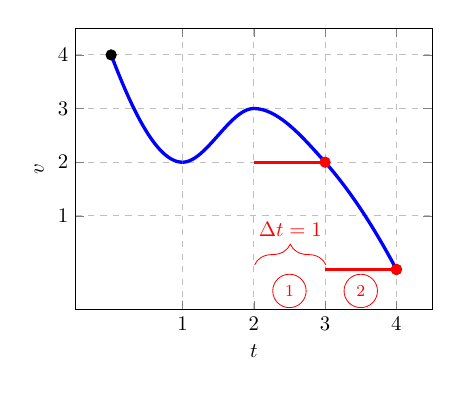
\begin{tikzpicture}[scale=0.75]
          \begin{axis}[
        %    axis y line = left,
        %    axis x line = bottom,
            xlabel = {$t$},
            ylabel = {$v$},
            xtick       = {1,2,3,4},
            xticklabels = {$1$,$2$,$3$,$4$},
            ytick       = {-2,-1,1,2,3,4,5,6},
            yticklabels = {$-2$,$-1$,$1$,$2$,$3$,$4$,$5$,$6$},
            samples     = 320,
            domain      = 0:4,
            %restrict y to domain=-5:5,
            xmin = -0.5, xmax = 4.5,
            ymin = -0.75, ymax = 4.5,
            width=3in,height=2.5in,
            grid=both, grid style=dashed
          ]
               \addplot[blue, ultra thick, mark=none, smooth, domain=0:1]  {4-7* x/2 + x^2 + x^3/2};
          \addplot[blue, ultra thick, mark=none, smooth, domain=1:2]  {7 - 12*x + 9*x^2 - 2*x^3};
          \addplot[blue, ultra thick, mark=none, smooth, domain=2:3]  {-7 + 12*x - 9/2* x^2 + x^3/2};
          \addplot[blue, ultra thick, mark=none, smooth, domain=3:4]  {2 + 3*x/2 - x^2/2};
         %
         \filldraw (0,4) circle (2.5pt);
         %
         \filldraw (4,0) circle (2.5pt);
         \draw [decorate,decoration={brace,amplitude=+10pt},xshift=0.4pt,yshift=-0.4pt, red](2,.1) -- (3,.1) node[red,midway,yshift=0.6cm] { $\Delta t=1$};
\node[circle,draw, red]  at (2.5,-.4){\footnotesize $1$};
\node[circle,draw, red]  at (3.5,-.4){\footnotesize $2$};
 \addplot[red, ultra thick, mark=none, smooth, domain=2:3]  {2};
          \filldraw[red] (3,2) circle (2.5pt);
           \addplot[red, ultra thick, mark=none, smooth, domain=3:4]  {0};
          \filldraw[red] (4,0) circle (2.5pt);
         \end{axis}
    \end{tikzpicture}
       \vs{-.1} \captionof*{figure}{\bf \footnotesize{ Approach $\#2$:\\Right endpoints}}
       \end{minipage}
}\vs{-.4}
\blue{
\itemI{
\item {\em Approach $\#1$: Left endpoints}. In this approach we use the left endpoint of each subinterval to determine the velocity.  
\itemI{
\item Over subinterval $[2,3]$ the left endpoint is $t=2$. From the graph, we see the velocity is $v(2)=3$ and draw a constant line $y=3$ over the same subinterval.
\item Over subinterval $[3,4]$ the left endpoint is $t=3$. From the graph, we see the velocity is $v(3)=2$ and draw a constant line $y=2$ over the same subinterval.
}
Since the elapsed time over each subinterval is $\Delta t=1$ our Net Change is 
\al{
\Delta x&=\Delta x_1+\Delta x_2\\
\Delta x&=v(3)\cdot \Delta t + v(2)\cdot \Delta t\\
\Delta x&=3\cdot 1+2\cdot 1=5
}
\item {\em Approach $\#2$: Right endpoints}. In this approach we use the right endpoint of each subinterval to determine the velocity.  
\itemI{
\item Over subinterval $[2,3]$ the right endpoint is $t=3$. From the graph, we see the velocity is $v(3)=2$ and draw a constant line $y=2$ over the same subinterval.
\item Over subinterval $[3,4]$ the right endpoint is $t=4$. From the graph, we see the velocity is $v(4)=0$ and draw a constant line $y=0$ over the same subinterval.
}
Since the elapsed time over each subinterval is $\Delta t=1$ our Net Change is 
\al{
\Delta x&=\Delta x_1+\Delta x_2\\
\Delta x&=v(2)\cdot \Delta t + v(0)\cdot \Delta t\\
\Delta x&=2\cdot 1+0\cdot 1=2
}
}
The {\em exact} Net Change is somewhere between $\Delta x=2$ and $\Delta x=5$.
}
\begin{enumerate}
\item[(b)] Given $t$ is assigned to the horizontal axis and $v$ is assigned to the vertical axis, how might we represent the quantity we computed in part (a) graphically? Sketch such a representation, and describe it in words below.
\end{enumerate}
\hs{-.5}\mpageT{.3}{.75}{
\begin{tikzpicture}[scale=0.75]
          \begin{axis}[
        %    axis y line = left,
        %    axis x line = bottom,
            xlabel = {$t$},
            ylabel = {$v$},
            xtick       = {1,2,3,4},
            xticklabels = {$1$,$2$,$3$,$4$},
            ytick       = {-2,-1,1,2,3,4,5,6},
            yticklabels = {$-2$,$-1$,$1$,$2$,$3$,$4$,$5$,$6$},
            samples     = 320,
            domain      = 0:4,
            %restrict y to domain=-5:5,
            xmin = -0.5, xmax = 4.5,
            ymin = -0.85, ymax = 4.5,
            width=3in,height=2.5in,
            grid=both, grid style=dashed
          ]
         %
	\draw [fill=red, opacity=0.2]  (2,3) rectangle (3,0); 
		\draw [fill=red, opacity=0.2]  (3,2) rectangle (4,0); 
               \addplot[blue, ultra thick, mark=none, smooth, domain=0:1]  {4-7* x/2 + x^2 + x^3/2};
          \addplot[blue, ultra thick, mark=none, smooth, domain=1:2]  {7 - 12*x + 9*x^2 - 2*x^3};
          \addplot[blue, ultra thick, mark=none, smooth, domain=2:3]  {-7 + 12*x - 9/2* x^2 + x^3/2};
          \addplot[blue, ultra thick, mark=none, smooth, domain=3:4]  {2 + 3*x/2 - x^2/2};
         %
         \filldraw (0,4) circle (2.5pt);
         %
         \filldraw (4,0) circle (2.5pt);
                  \draw [decorate,decoration={brace,amplitude=+10pt},xshift=0.4pt,yshift=-0.4pt, red](2,.1) -- (3,.1) node[red,midway,yshift=0.6cm] { \footnotesize $\Delta t=1$};
                                    \draw [decorate,decoration={brace,amplitude=+10pt},xshift=0.4pt,yshift=-0.4pt,  red](1.9,.0) -- (1.9,2.9) node[red,midway,xshift=-0.75cm] { $v(2)$};
\node[circle,draw, red]  at (2.5,-.4){\footnotesize $1$};
\node[circle,draw, red]  at (3.5,-.4){\footnotesize $2$};
 \addplot[red, ultra thick, mark=none, smooth, domain=2:3]  {3};
          \filldraw[red] (2,3) circle (2.5pt);
           \addplot[red, ultra thick, mark=none, smooth, domain=3:4]  {2};
          \filldraw[red] (3,2) circle (2.5pt);
          %%%%%%%%%
          	  \addplot[ name path=f1, domain=2:3,  blue, ultra thick,  ] {-7 + 12*x - 9/2* x^2 + x^3/2};
	   \path[name path=axis1] (2,0) -- (3,0);
	    \addplot [
                    thick,
                    color=blue!20,
                    fill=blue!20, 
                    ]
                    fill between[
                    of=f1 and axis1,
                    soft clip={domain=2:3},
                    ];
                %
           \addplot[ name path=f2, domain=3:4,  blue, ultra thick,  ] {2 + 3*x/2 - x^2/2};
	   \path[name path=axis2] (3,0) -- (4,0);
	    \addplot [
                    thick,
                    color=blue!20,
                    fill=blue!20, 
                    ]
                    fill between[
                    of=f2 and axis2,
                    soft clip={domain=3:4},
                    ];
                    %
         \end{axis}
    \end{tikzpicture}
}{
\sol{
$\Delta t$ is the width of each subinterval.  In our Left endpoint approach, we can think of $v(2)$ as the height of a rectangle over first subinterval. Thus we can interpret $$\Delta x_1=v(2)\cdot \Delta t$$ as the {\em area of the first rectangle}. Thus $$\Delta x=\Delta x_1+\Delta x_2= v(2)\cdot \Delta t+v(3)\cdot \Delta t$$
is the sum of areas of two rectangles and is an estimate of the {\em Net Area} between the graph of $v(t)$ and the horizontal axis over $2\leq t\leq 4$.
}
}
\begin{enumerate}
\item[(c)] $x(t)$ represents the position of the object from the origin at time $t$.  Based on your answer in part (a), if the object was at position $10$ meters at $2$ seconds after measurements were initially taken, then approximately where is the object $4$ seconds after measurements were taken?
\sol{
We are told $x(2)=10$. We want to find $x(4)$. We will add the Net Change of position to the initial position to find $x(4)$. In particular
\al{
x(4)&=x(2)+\Delta x\\
&=x(2)+\int_2^4v(t)\;dt\\
&\approx 10+5 \text{  (if using left endpoints).} \\
&=15 \text{ meters}
}
If we use right endpoints, then $x(4)\approx 10+2=12$ meters.
}


\end{enumerate}

%%%%%%%%%%%%%%%%%%%%%%%%%%%%%%%%%%%%%%%%%%%%%%%%%%%%%%%%%%%%%%%%%%%%%%%%%%%%%%%%%%%%%%%%%%%%%
\newpage%\end{document}%%%%%%%%%%%%%%%%%%%%%%%%%%%%%%%%%%%%%%%%%%%%%%%%%%%%%%%%%%%%%%%%%%%%%%%%%%%%%%%%%%%%
%%%%%%%%%%%%%%%%%%%%%%%%%%%%%%%%%%%%%%%%%%%%%%%%%%%%%%%%%%%%%%%%%%%%%%%%%%%%%%%%%%%%%%%%%%%%%

{\exercise}\ltrm{\bf\color{Fuchsia}I1} The weight, $w$ (in pounds), of a baby  is described by a function $w(t)$ where $t$ represents weeks after birth.  Below is a graph of the {\em growth rate} $w'(t)$ (in pounds per week) of an infant's weight $t$ weeks after birth. 
%
    \begin{minipage}[t][2in][t]{0.275\textwidth}
    \,\\[-0.1in]
    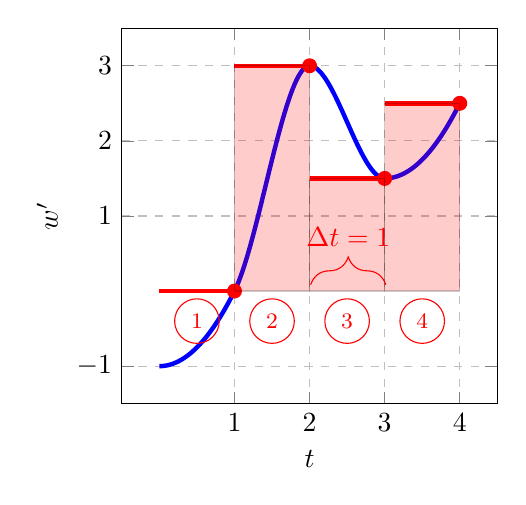
\begin{tikzpicture}
          \begin{axis}[
        %    axis y line = left,
        %    axis x line = bottom,
            xlabel = {$t$},
            ylabel = {$w'$},
            xtick       = {-2,-1,1,2,3,4,5,6},
            xticklabels = {$-2$,$-1$,$1$,$2$,$3$,$4$,$5$,$6$},
            ytick       = {-2,-1,1,2,3,4,5,6},
            yticklabels = {$-2$,$-1$,$1$,$2$,$3$,$4$,$5$,$6$},
            samples     = 320,
            domain      = -3:7,
            %restrict y to domain=-5:5,
            xmin = -0.5, xmax = 4.5,
            ymin = -1.5, ymax = 3.5,
            width=2.5in,height=2.5in,
            grid=both, grid style=dashed
          ]
         %
         % \addplot[blue, ultra thick, mark=none, smooth] coordinates{ (0,-1) (1,0) (2,3)  (3,1.5) (4,2.5)};
         %% In Mathematica, use ResourceFunction["CubicMonotonicInterpolation"][coords]. to find interpolating polynomial.
          \addplot[blue, ultra thick, mark=none, smooth, domain=0:1]  {x^2-1};
          \addplot[blue, ultra thick, mark=none, smooth, domain=1:2]  {7 - 20*x + 17*x^2 - 4* x^3};
          \addplot[blue, ultra thick, mark=none, smooth, domain=2:3]  {-39 + 54*x - 22.5*x^2 + 3* x^3};
          \addplot[blue, ultra thick, mark=none, smooth, domain=3:4]  {x^2-6*x+10.5};
         %
      	\filldraw[red] (1,0) circle (2.5pt);
	\addplot[red, ultra thick, mark=none, smooth, domain=0:1]  {0};
      	\filldraw[red] (2,3) circle (2.5pt);
	\addplot[red, ultra thick, mark=none, smooth, domain=1:2]  {3};
      	\filldraw[red] (3,1.5) circle (2.5pt);
	\addplot[red, ultra thick, mark=none, smooth, domain=2:3]  {1.5};
	\filldraw[red] (4,2.5) circle (2.5pt);
	\addplot[red, ultra thick, mark=none, smooth, domain=3:4]  {2.5};
	\draw [fill=red, opacity=0.2]  (1,3) rectangle (2,0); 
	\draw [fill=red, opacity=0.2]  (2,1.5) rectangle (3,0); 
	\draw [fill=red, opacity=0.2]  (3,2.5) rectangle (4,0); 
	\node[circle,draw, red]  at (0.5,-.4){\footnotesize $1$};
	\node[circle,draw, red]  at (1.5,-.4){\footnotesize $2$};
`	\node[circle,draw, red]  at (2.5,-.4){\footnotesize $3$};
	\node[circle,draw, red]  at (3.5,-.4){\footnotesize $4$};
	\draw [decorate,decoration={brace,amplitude=+10pt},xshift=0.4pt,yshift=-0.4pt, red](2,.1) -- (3,.1) node[red,midway,yshift=0.6cm] { $\Delta t=1$};
         \end{axis}
    \end{tikzpicture}
            \captionof*{figure}{\bf Right endpoints}
    \end{minipage}
    %decorate
    \quad
    %
 \begin{minipage}[t][2in][t]{0.625\textwidth}
        \begin{enumerate}
        \item[(a)] Estimate the net change $\Delta w$ in the infant's weight from birth to $4$ weeks. Sketch rectangles whose areas represent your estimate. ({\it Note:} There are many correct answers to this prompt!)\\
                \sol{
        The first choice to make is how many rectangles to use. There are many reasonable choices.   For this problem, we choose $n=4$ rectangles over the interval $0\leq t  \leq 4$.  This leads to
        \al{
        \Delta t&=\frac{end-start}{n}\\
        \Delta t&=\frac{4-0}{4}=4
        }
          }
        \end{enumerate}
    \end{minipage}
    ~\\\\\\
    \blue{{\bf Right endpoints}\\
         We also can use left endpoint rectangles, right endpoint rectangles, midpoint rectangles, or some other option. We will use right endpoint rectangles to illustrate this approach. There are $4$ subintervals so 
        \al{
        \Delta w&=\Delta w_1+\Delta w_2+\Delta w_3+\Delta w_4\\
        &=w^{\prime}(1)\cdot\Delta t+w^{\prime}(2)\cdot\Delta t+w^{\prime}(3)\cdot\Delta t+w^{\prime}(4)\cdot\Delta t\\&=0\cdot 1+3\cdot1+1.5\cdot 1+2.5\cdot 1\\
        &=7 \text{ $lbs.$}
        }
        ~\\
    \mpageT{.5}{.5}{
    {\bf Left Endpoints}
            \al{
        \Delta w&=\Delta w_1+\Delta w_2+\Delta w_3+\Delta w_4\\
        &=w^{\prime}(0)\cdot\Delta t+w^{\prime}(1)\cdot\Delta t+w^{\prime}(2)\cdot\Delta t+w^{\prime}(3)\cdot\Delta t\\
        &=-1\cdot 1+0\cdot1+3\cdot 1+1.5\cdot 1\\
        &=3.5 \text{ $lbs.$}
        }
   }{\centering
    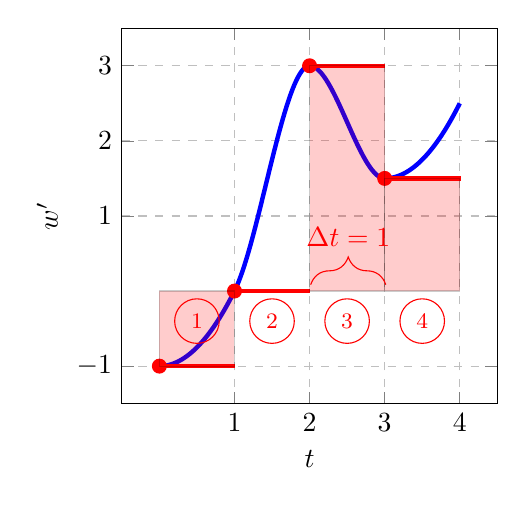
\begin{tikzpicture}
          \begin{axis}[
        %    axis y line = left,
        %    axis x line = bottom,
            xlabel = {$t$},
            ylabel = {$w'$},
            xtick       = {-2,-1,1,2,3,4,5,6},
            xticklabels = {$-2$,$-1$,$1$,$2$,$3$,$4$,$5$,$6$},
            ytick       = {-2,-1,1,2,3,4,5,6},
            yticklabels = {$-2$,$-1$,$1$,$2$,$3$,$4$,$5$,$6$},
            samples     = 320,
            domain      = -3:7,
            %restrict y to domain=-5:5,
            xmin = -0.5, xmax = 4.5,
            ymin = -1.5, ymax = 3.5,
            width=2.5in,height=2.5in,
            grid=both, grid style=dashed
          ]
         %
         % \addplot[blue, ultra thick, mark=none, smooth] coordinates{ (0,-1) (1,0) (2,3)  (3,1.5) (4,2.5)};
         %% In Mathematica, use ResourceFunction["CubicMonotonicInterpolation"][coords]. to find interpolating polynomial.
          \addplot[blue, ultra thick, mark=none, smooth, domain=0:1]  {x^2-1};
          \addplot[blue, ultra thick, mark=none, smooth, domain=1:2]  {7 - 20*x + 17*x^2 - 4* x^3};
          \addplot[blue, ultra thick, mark=none, smooth, domain=2:3]  {-39 + 54*x - 22.5*x^2 + 3* x^3};
          \addplot[blue, ultra thick, mark=none, smooth, domain=3:4]  {x^2-6*x+10.5};
         %
      	\filldraw[red] (0,-1) circle (2.5pt);
	\addplot[red, ultra thick, mark=none, smooth, domain=0:1]  {-1};
      	\filldraw[red] (1,0) circle (2.5pt);
	\addplot[red, ultra thick, mark=none, smooth, domain=1:2]  {0};
      	\filldraw[red] (2,3) circle (2.5pt);
	\addplot[red, ultra thick, mark=none, smooth, domain=2:3]  {3};
	\filldraw[red] (3,1.5) circle (2.5pt);
	\addplot[red, ultra thick, mark=none, smooth, domain=3:4]  {1.5};
	\draw [fill=red, opacity=0.2]  (0,-1) rectangle (1,0); 
	\draw [fill=red, opacity=0.2]  (2,3) rectangle (3,0); 
	\draw [fill=red, opacity=0.2]  (3,1.5) rectangle (4,0); 
	\node[circle,draw, red]  at (0.5,-.4){\footnotesize $1$};
	\node[circle,draw, red]  at (1.5,-.4){\footnotesize $2$};
`	\node[circle,draw, red]  at (2.5,-.4){\footnotesize $3$};
	\node[circle,draw, red]  at (3.5,-.4){\footnotesize $4$};
	\draw [decorate,decoration={brace,amplitude=+10pt},xshift=0.4pt,yshift=-0.4pt, red](2,.1) -- (3,.1) node[red,midway,yshift=0.6cm] { $\Delta t=1$};
         \end{axis}
    \end{tikzpicture}
    \captionof*{figure}{\bf Left endpoints}
}
~\\The actual net change in weight is probably between $3.5$ and $7$ lbs.
}

\begin{enumerate}
\item[(b)] Based on your answer in part (a), if the infant weighed 7 pounds at birth, then approximately how much did the infant weigh when the infant was 4 weeks old?
\sol{
Since the weight at birth (i.e. $t=0$) is $7$ lbs, we can say $$w(0)=7.$$ The weight after $4$ weeks is 
\al{
w(4)&= w(0)+\Delta w\\
&=7+3.5 \text{ (if we use the Left endpoint approach)}\\
&=10.5 \text{ $lbs.$}
}
}
\end{enumerate}
\vfill

\newpage
{\bf\color{blue}Mini-lecture.} ({\it net change, area, and the definite integral})

\hs{-.4}\mpageTfour{.25}{.25}{.25}{.35}{
    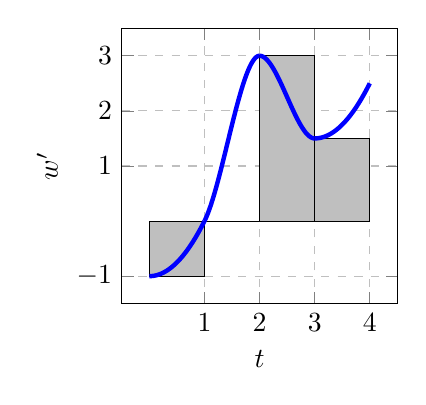
\begin{tikzpicture}
          \begin{axis}[
        %    axis y line = left,
        %    axis x line = bottom,
            xlabel = {$t$},
            ylabel = {$w'$},
            xtick       = {-2,-1,1,2,3,4,5,6},
            xticklabels = {$-2$,$-1$,$1$,$2$,$3$,$4$,$5$,$6$},
            ytick       = {-2,-1,1,2,3,4,5,6},
            yticklabels = {$-2$,$-1$,$1$,$2$,$3$,$4$,$5$,$6$},
            samples     = 320,
            domain      = -3:7,
            %restrict y to domain=-5:5,
            xmin = -0.5, xmax = 4.5,
            ymin = -1.5, ymax = 3.5,
            width=2in,height=2in,
            grid=both, grid style=dashed
          ]
         %
            \draw [fill=lightgray]  (3,1.5) rectangle (4,0); 
         \draw [fill=lightgray]  (2,3) rectangle (3,0); 
            \draw [fill=lightgray] (1,0) rectangle (2,0); 
            \draw [fill=lightgray] (0,-1) rectangle (1,0.0); 
         % \addplot[blue, ultra thick, mark=none, smooth] coordinates{ (0,-1) (1,0) (2,3)  (3,1.5) (4,2.5)};
         %% In Mathematica, use ResourceFunction["CubicMonotonicInterpolation"][coords]. to find interpolating polynomial.
          \addplot[blue, ultra thick, mark=none, smooth, domain=0:1]  {x^2-1};
          \addplot[blue, ultra thick, mark=none, smooth, domain=1:2]  {7 - 20*x + 17*x^2 - 4* x^3};
          \addplot[blue, ultra thick, mark=none, smooth, domain=2:3]  {-39 + 54*x - 22.5*x^2 + 3* x^3};
          \addplot[blue, ultra thick, mark=none, smooth, domain=3:4]  {x^2-6*x+10.5};
         %
         \end{axis}
    \end{tikzpicture}
    }{
    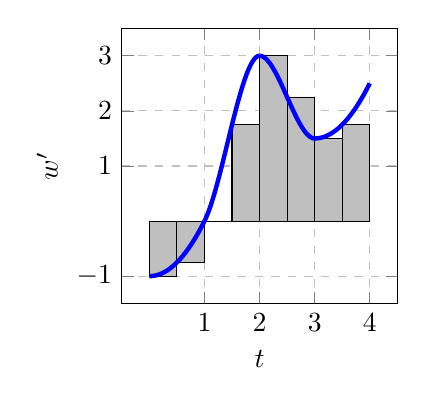
\begin{tikzpicture}
          \begin{axis}[
        %    axis y line = left,
        %    axis x line = bottom,
            xlabel = {$t$},
            ylabel = {$w'$},
            xtick       = {-2,-1,1,2,3,4,5,6},
            xticklabels = {$-2$,$-1$,$1$,$2$,$3$,$4$,$5$,$6$},
            ytick       = {-2,-1,1,2,3,4,5,6},
            yticklabels = {$-2$,$-1$,$1$,$2$,$3$,$4$,$5$,$6$},
            samples     = 320,
            domain      = -3:7,
            %restrict y to domain=-5:5,
            xmin = -0.5, xmax = 4.5,
            ymin = -1.5, ymax = 3.5,
            width=2in,height=2in,
            grid=both, grid style=dashed
          ]
         %
         \draw [fill=lightgray] (3.5,1.75) rectangle (4,0);
            \draw [fill=lightgray]  (3,1.5) rectangle (3.5,0); 
            \draw [fill=lightgray] (2.5,2.25) rectangle (3,0);
         \draw [fill=lightgray]  (2,3) rectangle (2.5,0); 
         \draw [fill=lightgray] (1.5,1.75) rectangle (2,0);
            \draw [fill=lightgray] (1,0) rectangle (1.5,0); 
            \draw [fill=lightgray] (.5,-.75) rectangle (1,0);
            \draw [fill=lightgray] (0,-1) rectangle (.5,0); 
         % \addplot[blue, ultra thick, mark=none, smooth] coordinates{ (0,-1) (1,0) (2,3)  (3,1.5) (4,2.5)};
         %% In Mathematica, use ResourceFunction["CubicMonotonicInterpolation"][coords]. to find interpolating polynomial.
          \addplot[blue, ultra thick, mark=none, smooth, domain=0:1]  {x^2-1};
          \addplot[blue, ultra thick, mark=none, smooth, domain=1:2]  {7 - 20*x + 17*x^2 - 4* x^3};
          \addplot[blue, ultra thick, mark=none, smooth, domain=2:3]  {-39 + 54*x - 22.5*x^2 + 3* x^3};
          \addplot[blue, ultra thick, mark=none, smooth, domain=3:4]  {x^2-6*x+10.5};
         %
         \end{axis}
    \end{tikzpicture}
    }{
        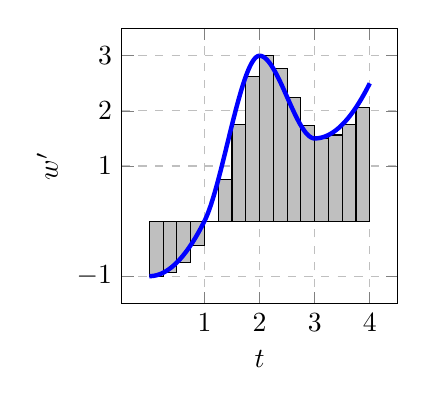
\begin{tikzpicture}
          \begin{axis}[
        %    axis y line = left,
        %    axis x line = bottom,
            xlabel = {$t$},
            ylabel = {$w'$},
            xtick       = {-2,-1,1,2,3,4,5,6},
            xticklabels = {$-2$,$-1$,$1$,$2$,$3$,$4$,$5$,$6$},
            ytick       = {-2,-1,1,2,3,4,5,6},
            yticklabels = {$-2$,$-1$,$1$,$2$,$3$,$4$,$5$,$6$},
            samples     = 320,
            domain      = -3:7,
            %restrict y to domain=-5:5,
            xmin = -0.5, xmax = 4.5,
            ymin = -1.5, ymax = 3.5,
            width=2in,height=2in,
            grid=both, grid style=dashed
          ]
         %
           \draw [fill=lightgray] (3.75,2.0625 ) rectangle (4,0);
         \draw [fill=lightgray] (3.5,1.75) rectangle (3.75,0);
           \draw [fill=lightgray] (3.25,1.5625 ) rectangle (3.5,0);
            \draw [fill=lightgray]  (3,1.5) rectangle (3.25,0); 
              \draw [fill=lightgray] (2.75,1.73438 ) rectangle (3,0);
            \draw [fill=lightgray] (2.5,2.25) rectangle (2.75,0);
              \draw [fill=lightgray] (2.25,2.76563 ) rectangle (2.5,0);
         \draw [fill=lightgray]  (2,3) rectangle (2.25,0); 
           \draw [fill=lightgray] ( 1.75,2.625) rectangle (2,0);
         \draw [fill=lightgray] (1.5,1.75) rectangle (1.75,0);
           \draw [fill=lightgray] ( 1.25,.75) rectangle (1.5,0);
            \draw [fill=lightgray] (1,0) rectangle (1.25,0); 
              \draw [fill=lightgray] ( .75,-.4375) rectangle (1,0);
            \draw [fill=lightgray] (.5,-.75) rectangle (.75,0);
             \draw [fill=lightgray] ( .25,-.9375) rectangle (.5,0);
            \draw [fill=lightgray] (0,-1) rectangle (.25,0); 
         % \addplot[blue, ultra thick, mark=none, smooth] coordinates{ (0,-1) (1,0) (2,3)  (3,1.5) (4,2.5)};
         %% In Mathematica, use ResourceFunction["CubicMonotonicInterpolation"][coords]. to find interpolating polynomial.
          \addplot[blue, ultra thick, mark=none, smooth, domain=0:1]  {x^2-1};
          \addplot[blue, ultra thick, mark=none, smooth, domain=1:2]  {7 - 20*x + 17*x^2 - 4* x^3};
          \addplot[blue, ultra thick, mark=none, smooth, domain=2:3]  {-39 + 54*x - 22.5*x^2 + 3* x^3};
          \addplot[blue, ultra thick, mark=none, smooth, domain=3:4]  {x^2-6*x+10.5};
         %
         \end{axis}
    \end{tikzpicture}
    }{%%startherex
    \mpage{.5}{.714}{\centering
    \blue{
    $n=\# rectangles$\\
    {\large $\ds \limn \longrightarrow$}
    }
    }{
    \begin{flushright}
            \begin{tikzpicture}
          \begin{axis}[
        %    axis y line = left,
        %    axis x line = bottom,
            xlabel = {$t$},
            ylabel = {$w'$},
            xtick       = {-2,-1,1,2,3,4,5,6},
            xticklabels = {$-2$,$-1$,$1$,$2$,$3$,$4$,$5$,$6$},
            ytick       = {-2,-1,1,2,3,4,5,6},
            yticklabels = {$-2$,$-1$,$1$,$2$,$3$,$4$,$5$,$6$},
            samples     = 320,
            domain      = -3:7,
            %restrict y to domain=-5:5,
            xmin = -0.5, xmax = 4.5,
            ymin = -1.5, ymax = 3.5,
            width=2in,height=2in,
            grid=both, grid style=dashed
          ]
         %
         % \addplot[blue, ultra thick, mark=none, smooth] coordinates{ (0,-1) (1,0) (2,3)  (3,1.5) (4,2.5)};
         %% In Mathematica, use ResourceFunction["CubicMonotonicInterpolation"][coords]. to find interpolating polynomial.
          \addplot[blue, ultra thick, mark=none, smooth, domain=0:1]  {x^2-1};
          \addplot[blue, ultra thick, mark=none, smooth, domain=1:2]  {7 - 20*x + 17*x^2 - 4* x^3};
          \addplot[blue, ultra thick, mark=none, smooth, domain=2:3]  {-39 + 54*x - 22.5*x^2 + 3* x^3};
          \addplot[blue, ultra thick, mark=none, smooth, domain=3:4]  {x^2-6*x+10.5};
         %
         \addplot[ name path=f1, domain=0:1,  blue, ultra thick,  ] {x^2-1};
	   \path[name path=axis1] (0,0) -- (1,0);
	    \addplot [
                    thick,
                    color=lightgray,
                    fill=lightgray, 
                    ]
                    fill between[
                    of=f1 and axis1,
                    soft clip={domain=0:1},
                    ];
                    %
	\addplot[ name path=f2, domain=1:2,  blue, ultra thick,  ] {7 - 20*x + 17*x^2 - 4* x^3};
	   \path[name path=axis2] (1,0) -- (2,0);
	    \addplot [
                    thick,
                    color=lightgray,
                    fill=lightgray, 
                    ]
                    fill between[
                    of=f2 and axis2,
                    soft clip={domain=1:2},
                    ];
	\addplot[ name path=f3, domain=2:3,  blue, ultra thick,  ] {-39 + 54*x - 22.5*x^2 + 3* x^3};
	   \path[name path=axis3] (2,0) -- (3,0);
	    \addplot [
                    thick,
                    color=lightgray,
                    fill=lightgray, 
                    ]
                    fill between[
                    of=f3 and axis3,
                    soft clip={domain=2:3},
                    ];
	\addplot[ name path=f4, domain=3:4,  blue, ultra thick,  ] {x^2-6*x+10.5};
	   \path[name path=axis4] (3,0) -- (4,0);
	    \addplot [
                    thick,
                    color=lightgray,
                    fill=lightgray, 
                    ]
                    fill between[
                    of=f4 and axis4,
                    soft clip={domain=3:4},
                    ];
         \end{axis}
    \end{tikzpicture}
    \end{flushright}
    }
    }
\blue{
Notice that the more rectangles that are used,  the smaller the ``gaps" we see between the graph of $w^{\prime}(t)$ and the rectangles. This means our estimate of Net Area/Net Change is getting better and better as we increase the number of rectangles. If we take a limit to infinity. We get the {\em Exact Net Area} or {\em Exact Net Change}. This Exact Net Area/Change is such an incredibly important idea that we give it it's own special symbol:
$$\text{\em Exact Net Area/Change}=\int_0^4 w^{\prime}(t)\;dt$$
}
\newpage
\important{The Definite Integral}
{
Let $a$ and $b$ be real numbers with $a<b$, and suppose $f$ is continuous on the interval $[a,b]$. The {\bf definite integral} of $f$ from $a$ to $b$ is denoted by \[\int_a^b f(x)\,dx\] and represents the \unline{1}{\blue{Net Area}}{.25} between the graph of $f$ and the interval along the $x$-axis from $a$ to $b$. If $f$ represents the rate of change of a quantity, then $\ds \int_a^b f(x)\,dx$ represents the \unline{1.5}{\blue{Net Change}}{.25} in the quantity as $x$ varies from $a$ to $b$.
}
\example Based on the definition of definite integral, write down a mathematical expression representing the net change $\Delta w$ in the infant's weight from birth to 4 weeks for the scenario in Exercise A, and indicate its units.
\sol{
$$\int_0^4 w^{\prime}(t)\;dt \text{ pounds}$$ 
}
\exercise\ltrm{\bf\color{Fuchsia}I1} Let $T'(t)$ represent the (instantaneous) rate of change (in $^{\circ}$C/day) of temperature in Charlottesville at a time $t$ (in days) during a particular week. 

\begin{enumerate}
\item[(a)] What are the units of $\ds \int_{1/2}^{3/2} T'(t)\,dt$? 
\sol{
Degrees Celsius, $^\circ C$
}

\item[(b)] What does this integral represent in the given context?
\sol{
The net change in the temperature (in degrees Celsius) between noon on Day 1 (i.e. $t=1/2$) to noon on Day 2 (i.e. $t=3/2$)
}
%\hfill ({\small\it continued on next page})

%%%%%%%%
%%%%%%%%%
%%%%%%%%%%
%%%%%%%%%%%
%\newpage%%%
%%%%%%%%%%%
%%%%%%%%%%
%%%%%%%%%
%%%%%%%%

\item[(c)] \pe If the temperature at noon on the first day of the week is $20^{\circ}$ C, then which of the following integral expressions represents the temperature at noon on the second day of the week?
   \enumAA{
        \item $20+\ds \int_{1/2}^{3/2} T'(t)\,dt$ \blue{\bf Correct!}
        \item $20-\ds \int_{1/2}^{3/2} T'(t)\,dt$
        \item $\ds \int_{1/2}^{3/2} T'(t)\,dt-20$
        \item $\ds \int_{0}^{3/2} T'(t)\,dt$
        \item None of these options.
   }
   \sol{
   The temperature at noon on the second day of the week, $T(3/2)$, will be
   \al{
   T(3/2)&=\text{temperature at noon on Day 1 $+$ net change in temperature}\\
   T(3/2)&=T(1/2)+\Delta T\\
   T(3/2)&=T(1/2)+\int_{1/2}^{3/2}T^{\prime}(t)\;dt\\
   T(3/2)&=20+\int_{1/2}^{3/2}T^{\prime}(t)\;dt\\
   }
   Thus choice A is the best choice.
   }
\end{enumerate}

\newpage
{\exercise}\ltrm{\bf\color{Fuchsia}I1} The population of a country changes over time as people immigrate and emigrate. Suppose $f(t)$ gives the rate of change of the population $t$ years after officials began keeping records, in thousands per year. The graph of $f$ is given below.\\

\begin{minipage}[t]{0.3\textwidth}
\,\\[-0.1in]
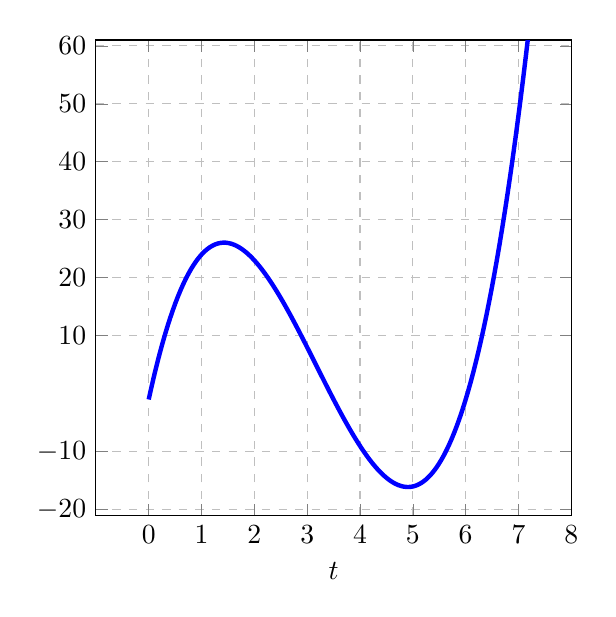
\begin{tikzpicture}
  \begin{axis}[
%    axis y line = left,
%    axis x line = bottom,
    xlabel = {$t$},
    %ylabel = { },
    xtick       = {0,1,2,3,4,5,6,7,8},
    xticklabels = {$0$,$1$,$2$,$3$,$4$,$5$,$6$,$7$,$8$},
    ytick       = {-20,-10,10,20,30,40,50,60},
    %yticklabels = {},
    samples     = 160,
    domain      = -1:3,
    restrict y to domain=-20:100,
    xmin = -1, xmax = 8,
    ymin = -21, ymax = 61,
    width = 3in, height=3in,
    grid=both, grid style=dashed
  ]
  \addplot[domain=0:8, blue, ultra thick] {-1+42*x-19*x^2+2*x^3};
\end{axis}
\end{tikzpicture}
\end{minipage}
%
\hfill
%
\begin{minipage}[t]{0.6\textwidth}
\begin{enumerate}
\item[(a)] Interpret in words the meaning of each of the following in terms of the context described above, including units.
    \begin{enumerate}
    \item[i.] $f(1)=24$
\sol{
The population is increasing at a rate of 24000 people per year at the end of year 1. \\\\
{\em Alternative Description:} If the population were to continue to change exactly as it did at the end of year 1, then the population would increase by 24 people per year. (IROC)
}
    \item[ii.] $\ds \int_1^7 f(t)\,dt$
    \sol{
    From the end of year 1 to the end of year 7, the population of this country grew by 36000 people.
    }
    \end{enumerate}
\end{enumerate}
\end{minipage}

\begin{enumerate}
\item[(b)] Use 3 rectangles to estimate $\ds \int_1^7 f(t)\,dt$. Sketch rectangles whose areas represent your estimate. Note: There are many reasonable ways to do this!
\sol{~\\
\mpageT{.7}{.3}{
{\bf Left endpoints}  There are several reasonable approaches. We will use Left Endpoints.
\itemI{
\item $n=3$ rectangles means $\ds \Delta t=\frac{end-start}{n}=\frac{7-1}{3}=2$
\item Left endpoints occur at $t=1$, $t=3$ and $t=5$.
\item If $P(t)$ represents the population $t$ years after starting to keep records, 
\al{\ds \Delta P=\int_1^7 f(t)\,dt &\approx f(1)\cdot \Delta t+f(3)\cdot \Delta t+f(5)\cdot \Delta t\\
&=24\cdot 2+8\cdot 2+ ^-16\cdot 2 \text{ (values for $f(t)$ estimated from graph)}\\
&=32
}
Thus the net change in population between years $1$ and $7$ is approximately $32,000$ people.
}
}{
%%%Start2here
   \begin{flushright}
   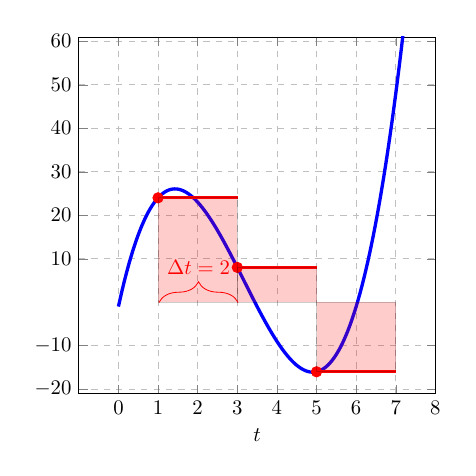
\begin{tikzpicture}[scale=.75]
  \begin{axis}[
%    axis y line = left,
%    axis x line = bottom,
    xlabel = {$t$},
    %ylabel = { },
    xtick       = {0,1,2,3,4,5,6,7,8},
    xticklabels = {$0$,$1$,$2$,$3$,$4$,$5$,$6$,$7$,$8$},
    ytick       = {-20,-10,10,20,30,40,50,60},
    %yticklabels = {},
    samples     = 160,
    domain      = -1:3,
    restrict y to domain=-20:100,
    xmin = -1, xmax = 8,
    ymin = -21, ymax = 61,
    width = 3in, height=3in,
    grid=both, grid style=dashed
  ]
  \addplot[domain=0:8, blue, ultra thick] {-1+42*x-19*x^2+2*x^3};
  \filldraw[red] (1,24) circle (2.5pt);
  \addplot[red, ultra thick, mark=none, smooth, domain=1:3]  {24};
  \filldraw[red] (3,8) circle (2.5pt);
  \addplot[red, ultra thick, mark=none, smooth, domain=3:5]  {8};
  \filldraw[red] (5,-16) circle (2.5pt);
  \addplot[red, ultra thick, mark=none, smooth, domain=5:7]  {-16};\
  \draw [fill=red, opacity=0.2]  (1,24) rectangle (3,0); 
  \draw [fill=red, opacity=0.2]  (3,8) rectangle (5,0); 
  \draw [fill=red, opacity=0.2]  (5,-16) rectangle (7,0); 
  \draw [decorate,decoration={brace,amplitude=+10pt},xshift=0.4pt,yshift=-0.4pt, red](1,.1) -- (3,.1) node[red,midway,yshift=0.6cm] { $\Delta t=2$};
\end{axis}
\end{tikzpicture}
\end{flushright} 
}
\mpageT{.7}{.3}{
{\bf Right endpoints}  A second reasonable approach would be to use Right Endpoints.
\itemI{
\item $n=3$ rectangles means $\ds \Delta t=\frac{end-start}{n}=\frac{7-1}{3}=2$
\item Right endpoints occur at  $t=3$, $t=5$, and $t=7$.
\item If $P(t)$ represents the population $t$ years after starting to keep records, 
\al{\ds \Delta P=\int_1^7 f(t)\,dt &\approx f(3)\cdot \Delta t+f(5)\cdot \Delta t +f(7_\cdot \Delta t\\
&=8\cdot 2+ ^-16\cdot 2 +48\cdot 2 \text{ (values for $f(t)$ estimated from graph)}\\
&=80
}
Thus the net change in population between years $1$ and $7$ is approximately $80,000$ people.
}
}{
   \begin{flushright}
   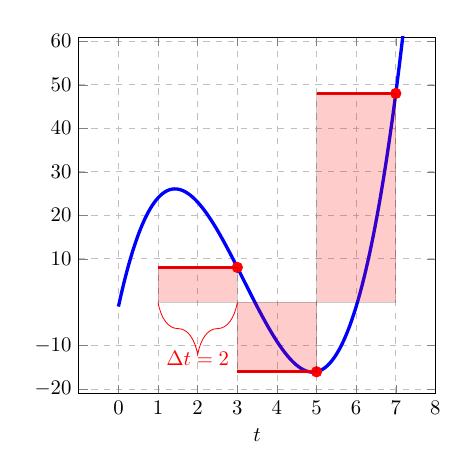
\begin{tikzpicture}[scale=.75]
  \begin{axis}[
%    axis y line = left,
%    axis x line = bottom,
    xlabel = {$t$},
    %ylabel = { },
    xtick       = {0,1,2,3,4,5,6,7,8},
    xticklabels = {$0$,$1$,$2$,$3$,$4$,$5$,$6$,$7$,$8$},
    ytick       = {-20,-10,10,20,30,40,50,60},
    %yticklabels = {},
    samples     = 160,
    domain      = -1:3,
    restrict y to domain=-20:100,
    xmin = -1, xmax = 8,
    ymin = -21, ymax = 61,
    width = 3in, height=3in,
    grid=both, grid style=dashed
  ]
  \addplot[domain=0:8, blue, ultra thick] {-1+42*x-19*x^2+2*x^3};
  \filldraw[red] (3,8) circle (2.5pt);
  \addplot[red, ultra thick, mark=none, smooth, domain=1:3]  {8};
    \filldraw[red] (5,-16) circle (2.5pt);
  \addplot[red, ultra thick, mark=none, smooth, domain=3:5]  {-16};
    \filldraw[red] (7,48) circle (2.5pt);
  \addplot[red, ultra thick, mark=none, smooth, domain=5:7]  {48};
  \draw [fill=red, opacity=0.2]  (1,8) rectangle (3,0); 
  \draw [fill=red, opacity=0.2]  (3,-16) rectangle (5,0); 
  \draw [fill=red, opacity=0.2]  (5,48) rectangle (7,0); 
  \draw [decorate,decoration={brace,amplitude=+25pt},xshift=0pt,yshift=+0pt, red] (3,-.1) -- (1,-.1) node[red,midway,yshift=-0.95cm] { $\Delta t=2$};
\end{axis}
\end{tikzpicture}
\end{flushright} 
}
}
\item[(c)] Suppose the population $1$ year after officials began keeping records was $2000$. Write $-$ but do not solve $-$ an integral expression representing the number of people at time $t=4$.
\sol{
The population at $t=4$ is the initial population at $t=1$ plus the net change in population between years $t=1$ and $t=4$. Thus
\al{
P(4)&=P(1)+\Delta P\\
P(4)&=P(1)+\int_1^4f(t)\;dt\\
P(4)&=2+\int_1^4f(t)\;dt \text{ (since units are thousands, $2$ represents $2,000$ people)}\\
}
}

\end{enumerate}


%%%%%%%%
%%%%%%%%%
%%%%%%%%%%
%%%%%%%%%%%
\newpage%%%
%%%%%%%%%%%
%%%%%%%%%%
%%%%%%%%%
%%%%%%%%


{\bf\color{blue}Extra Practice 1.}\ltrm{\bf\color{Fuchsia}I1} A faucet is pouring water into a tank, which happens to have a small hole in the bottom. Suppose $r(t)$ is the rate at which the volume of water in the tank is changing, measured in gallons per hour, $t$ hours after the faucet is turned on.
    \begin{enumerate}
    \item[(a)] Interpret in words the meaning of each of the following in the given context, including units.
        \begin{enumerate}
        \item[i.] $r(2)=-1$
\sol{
Two hours after the faucet is turned on, the water volume is {\em decreasing} at a rate of 1 gallon per hour.\\\\
{\em Alternative Description:} If the volume of water were to continue to change exactly as it did two hours after the faucet is turned on, then the water volume would decrease by 1 gallon per hour. (IROC)
}
        \item[ii.] $\ds \int_1^3 r(t)\,dt$
\sol{
This represents how much the volume of water (in gallons) in the tank changed from 1 hour to 3 hours after the faucet is turned on.
}
        \end{enumerate}

    \item[(b)] Write a mathematical expression representing the following.
        \begin{enumerate}
        \item[i.] the net change (in gallons) in the amount of water in the bucket two hours after the faucet is turned on
\sol{ Net change from $t=0$ to $t=2$: 
$$\int_0^2 r(t)\, dt$$
}

        \item[ii.] the initial rate (in gallons per hour) at which the volume of water in the tank is changing   
\sol{ We assume that the initial rate occurs at $t=0$. Thus the initial rate the at which the volume of water in the tank is changing is
$$r(0)$$
}
        \end{enumerate}

    \item[(c)] Suppose the tank initially contains $1$ gallon of water. Write an integral expression representing the amount of water in the bucket $2$ hours after the faucet is turned on.
\sol{Volume at  $t=2$: 
$$1 + \int_0^2 r(t)\, dt$$
}
    \end{enumerate}

\end{document}
